\section{Einleitung}\label{sec:einleitung}
Innovationen entstehen aus Ideen. Ideen gibt es sehr viele. Doch nicht jede Idee ist sinnvoll umsetzbar.
Ein Beispiel ist ein Produkt des bekannten Zahnpastaherstellers Colgate. 
Dessen \textit{Beef Lasagne} konnte sich nicht am Markt durchsetzen. 
Vermutlich zielte Colgate mit der Vermarktung der Lasagne ein neues Marktgebiet an. \\
Leider wurden die Kriterien für die Bewertung nicht gut gewählt, denn das Produkt passte nicht zum Unternehmens-Image.
Dies hatte zur Folge, dass sich das Produkt nicht verkaufte und sich als Marketing-Flop herausstellte.
\begin{figure}[h]
	\centering
	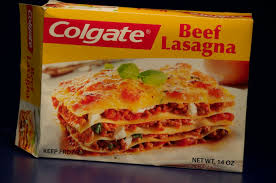
\includegraphics[width=6cm]{colgate.jpg}
	\caption{Beef Lasagne von Colgate}
	\label{img:colgate}
\end{figure}
Dieses Beispiel zeigt, wie wichtig es ist, Ideen anhand verschiedener Kriterien zu bewerten. 
In dieser Seminararbeit werden die Definitionen von Zephram und Schawel-Billig erläutert. \\
Zusätzlich werden anhand 
von zwei Praxisbeispielen Anwendungsfälle dargestellt und deren Kriterien zur Ideenbewertung beschrieben.